%===================================================================================
% Chapter: Extracción de Información
%===================================================================================
\chapter{Extracción de Información}\label{chapter:information_extraction}
\addcontentsline{toc}{chapter}{Extracción de Información}

\section{Extracción de Entidades}

Una entidad nombrada es una palabra o frase que identifica un objeto de un conjunto de objetos que tienen atributos similares. Ejemplos de esto son las personas, las organizaciones, drogas, nombres de enfermedades dentro del dominio m\'edico, entre otros. \textbf{Reconocimiento de Entidades Nombradas} (\textbf{NER}) es el proceso de localizar y clasificar entidades nombradas en un texto dentro de un conjunto de categor\'ias predefinidas de entidades.
Formalmente, dada una secuencia de \emph{tokens} $s=<w_1, w_2, ..., w_N >$, \textbf{NER} devuelve como salida una lista de tuplas $<I_s, I_e, t>$, una por cada entidad mencionada en s, donde $I_s \in [1,...,N]$ y $I_e \in [1,...,N]$ son el inicio y el fin de los \'indices de la entidad nombrada mencionada; y $t$ es el tipo de la misma dentro de una categor\'ia predefinida~\cite{li2018survey}. 

\textbf{NER} es un paso importante de preprocesamiento para una variedad de problemas tales como \emph{Recuperaci\'on de Informaci\'on}, \emph{Preguntas y Respuestas}, \emph{Traducci\'on de m\'aquina}, etc.


\subsection{Enfoque Basado en Reglas}

Los sistemas de \textbf{NER} basados en reglas dependen de \emph{hand-crafted rules}. Las reglas pueden ser dise\~nadas basadas en el dominio espec\'ifico \emph{gazetteers}~\cite{etzioni2005unsupervised},~\cite{sekine2004definition} y en patrones sint\'acticos-l\'exicos~\cite{zhang2013unsupervised}. En el dominio biom\'edico~\cite{hanisch2005prominer} se propuso \emph{ProMiner} el cual utiliza un diccionario de sin\'onimos preprocesado para identificar prote\'inas en texto biom\'edico.

Otros sistemas de \textbf{NER} basados en reglas conocidos son \textbf{LaSIE-II}~\cite{humphreys1998university}, \textbf{NetOwl}~\cite{krupka2005description}, \textbf{Facile}~\cite{black1998facile} y \textbf{SAR}~\cite{aone1998sra}. Todos estos sistemas consisten esencialmente en \emph{hand-crafted semantic} y reglas sint\'acticas para reconocer entidades. Los sistemas basados en reglas trabajan bien cuando el lexicon es exhaustivo, a su vez con las reglas de dominio espec\'ifico y diccionarios incompletos, alta precisi\'on y bajo recobrdado son comunmente observados en estos sistemas. Adem\'as estos sistemas no pueden ser trasnferidos a otros dominios~\cite{li2018survey}.


\subsection{Enfoques de Aprendizaje no Supervisado}  

Uno de los t\'ipicos enfoques de \textbf{Aprendizaje no Supervisado} es \emph{clustering}~\cite{nadeau2007survey}. Los sistemas de \textbf{NER} basados en \emph{clustering} extraen entidades nombradas de los distintos \emph{clusters} basado en las similiridades del contexto. La idea esencial es que recursos l\'exicos, patrones l\'exicos y estad\'isticas computadas en grandes \emph{corpus} pueden ser utilizadas para inferir entidades nombradas~\cite{li2018survey}. Collins~\cite{collins1999unsupervised} observ\'o que el uso de datos no etiquetados reduce los requerimientos para la supervision a solo 7 simples reglas. Similarmente, el sistema \textbf{KNOWITALL}~\cite{etzioni2005unsupervised} leverage un conjunto de nombres de predicados como entrada y \emph{bootstrap} el proceso de reconocimiento desde un conjunto peque\~no de patrones gen\'ericos de extracci\'on.

Un sistema no supervisado para la construcci\'on de \emph{gazetteers} y la resoluci\'on de la ambiguedad entre entidades nombradas fue presentado por~\cite{nadeau2006unsupervised}. Este sistema combina \textbf{NER} y la 
desambiguación de las entidades, basado en simples heur\'isticas que son efectivas a\'un. Enfoques no supervisados para el \textbf{NER} en textos biom\'edicos ha sido presentado por~\cite{zhang2013unsupervised}, donde su modelo depende de terminolog\'ias, estad\'isticas en \emph{corpus}~(la frecuencia de documentos inversa y vectores de contexto) y \emph{shallow syntactic knowledge} (e.g, noun phrase chunking). Los experimentos en dos conjuntos de datos biom\'edicos demuestran la efectividad y capacidad de generalizaci\'on de su enfoque no supervisado.


\subsection{Enfoque de Aprendizaje Supervisado Basado en Rasgos}

Cuando se aplica \textbf{Aprendizaje Supervisado}, el problema de \textbf{NER} consiste en una tarea de multiclasificaci\'on o etiquetado de secuencias. Donde dados, ejemplos anotados y rasgos dise\~nados para representar cada ejemplo entrenante, los algoritmos de aprendizaje de m\'aquinas son utilizados para aprender el modelo para reconocer patrones similares de datos no vistos~\cite{li2018survey}.

El dise\~no de rasgos es esencial en los sistemas supervisados de \textbf{NER}. La representaci\'on por un vector de rasgos es una abstracci\'on sobre el texto donde una palabra es representada por uno o muchos valores \emph{booleanos}, \emph{num\'ericos} o nominales~\cite{nadeau2007survey},~\cite{sekine2009named}. Existen rasgos a nivel de palabras (e.g \emph{case}, morfolog\'ia y \emph{part-of-speech tag}~\cite{zhou2002named},~\cite{settles2004biomedical},~\cite{liao2009simple}), lista de \emph{lookup features}(e.g. \emph{Wikipedia} gazetteer y DBpedia gazetteer~\cite{mikheev1999knowledge},~\cite{hoffart2011robust}) y rasgos de documentos y corpus (e.g. sintaxis local  y m\'ultiples ocurrencias~\cite{ravin1997extracting},~\cite{zhu2005espotter},~\cite{ji2016joint},~\cite{krishnan2006effective}).

Utilizando estos rasgos muchos algoritmos de \emph{aprendizaje de m\'aquina} supervisados han sido aplicados en \textbf{NER}. Ejemplo de esto son \emph{Hidden Markov Models} (\textbf{HMM})~\cite{bikel1997nymble},~\cite{bikel1999algorithm}, \emph{Decision Trees}~\cite{quinlan1986induction},~\cite{szarvas2006multilingual}, \emph{Maximum Entropy Models}~\cite{kapur1989maximum},~\cite{borthwick1998nyu},~\cite{bender2003maximum},~\cite{chieu2002named},~\cite{curran2003language}, \emph{Support Vector Machines}(\textbf{SVM})~\cite{hearst1998support},~\cite{isozaki2002efficient},~\cite{li2004svm} y \emph{Conditional Random Fields}(\textbf{CRF})~\cite{settles2004biomedical},~\cite{lafferty2001conditional},~\cite{mccallum2003early},~\cite{ritter2011named},~\cite{liu2011recognizing},~\cite{rocktaschel2012chemspot}.

\subsection{Enfoque Basado en T\'ecnicas de Aprendizaje Profundo}
En los \'ultimos a\~nos modelos para \textbf{NER} basados en \textbf{Aprendizaje Profundo} se han vuelto dominante. En comparaci\'on con enfoques basados en rasgos, el \textbf{aprendizaje profundo} es capaz de descubrir rasgos ocultos autom\'aticamente~\cite{li2018survey}. La figura~\ref{fig:NerDeepBased} muestra la arquitectura general de un modelo de aprendizaje profundo enfocado a resolver el problema de \textbf{NER}. 

Existen 3 ventajas esenciales de aplicar t\'ecnicas de aprendizaje profundo para resolver \textbf{NER}. En primer lugar, \textbf{NER} se beneficia de la aplicaci\'on de transformaciones no lineares, lo cual genera mapeos no lineares de la \emph{entrada} hacia la \emph{salida}, a diferencia de modelos lienares como \textbf{HMM}. En segundo lugar, el aprendizaje profundo ahorra esfuerzo significativo para dise\~nar \textbf{NER} features. Y en tercer lugar, los modelos de aprendizaje profundo para \textbf{NER} pueden ser entrenados con un paradigma \emph{end-to-end}, usando descenso por gradiente~\cite{li2018survey}.

\begin{figure}[h!]
	\centering
	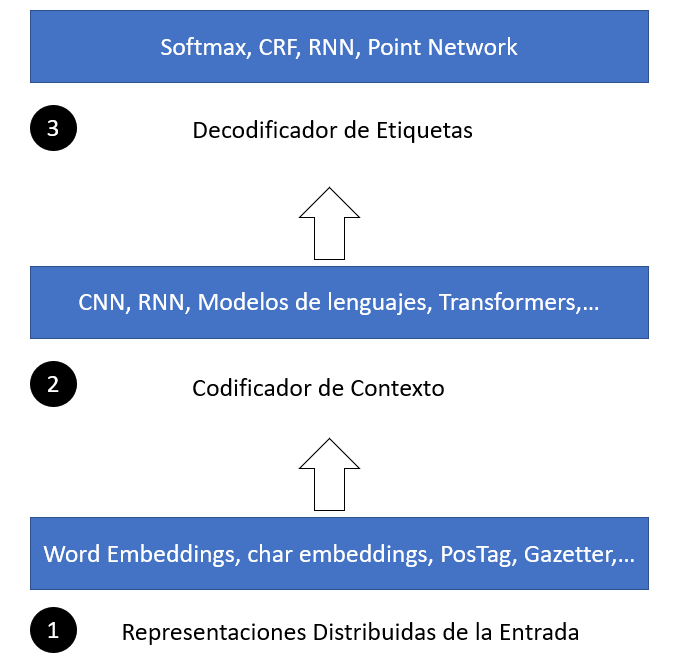
\includegraphics[width = 10cm]{Imagenes/NERDeep.png}
	\caption{Arquitectura general de aprendizaje profundo para NER.}\label{fig:NerDeepBased}
\end{figure}

\subsection{Representaci\'on Distribuida de la Entrada}

Una primera opci\'on para la representaci\'on de una palabra es el \emph{one-hot vector}. En el espacio de los \emph{one-hot vector}, dos palabras tienen completamente dos diferentes representaciones y son ortogonales. Las representaciones distribuidas representan palabras en vectores densos de valores reales con peque\~na dimensi\'on donde cada dimensi\'on representa un rasgo latente. Las representaciones distribuidas capturan propiedades sem\'anticas y sint\'acticas de la palabra.    

Algunos estudios~\cite{nguyen2016toward},~\cite{strubell2017fast} utilizan representaciones a nivel de palabras que son tipicamente pre-entrenadas sobre un largo n\'umero de colecciones de texto a trav\'es de algoritmos no supervisados tales como \emph{continuous bag of words (CBOW)} y \emph{continuous skip-gram models}~\cite{mikolov2013efficient}. En la figura~\ref{fig:cbowSkip} se muestra como \emph{CBOW} predice la palabra actual basada en el contexto y \emph{Skip-gram} predice las palabras del contexto dada la palabra actual. Estudios recientes como~\cite{yang2018design} han mostrado la importancia de los \emph{word embeddings} pre-entrenados. Entre los m\'as comunes se encuentran \emph{Word2Vec}~\footnote{https://code.google.com/archive/p/word2vec/} y \emph{GloVe}~\footnote{http://nlp.stanford.edu/projects/glove/}. En el caso de \textbf{NER} en el dominio biom\'edico se encuentra \textbf{Bio-NER}~\cite{yao2015biomedical}, donde la represenatci\'on de palabras del mismo es entrenado en la base de datos de \textbf{PubMed} usando un modelo \emph{skip-gram}. Otros trabajos que utilizan  representaciones a nivel de palabra son~\cite{zhai2017neural},~\cite{zhou2017joint},~\cite{ma2016end},~\cite{li2017leveraging},~\cite{wang2018code}.

\begin{figure}[h!]
	\centering
	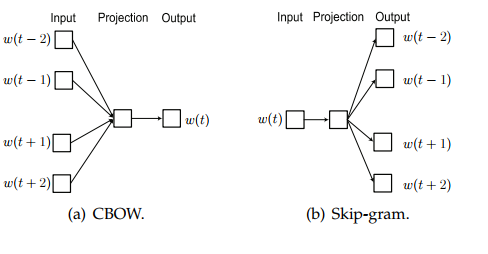
\includegraphics[width = 10cm]{Imagenes/CBOW_SkipGram.png}
	\caption{Arquitectura de CBOW y Skip-gram.}\label{fig:cbowSkip}
\end{figure}


Otra de las representaciones utilizadas en muchos estudios~\cite{kuru2016charner},~\cite{tran2017named},~\cite{li2018segbot} son las basadas en los caracteres de las palabras, la cual se aprende a partir de un modelo de redes neuronales \emph{end-to-end}. La representaci\'on a nivel de caracteres ha mostrado ser \'util para explotar informaci\'on por debajo del nivel de la palabra tales como prefijo y sufijos. Adem\'as posee la ventaja de otorgar una representaci\'on a las palabras que incluso no pertenezcan al vocabulario y compartir informaci\'on a nivel de regularidades y morfemas. Las dos arquitecturas m\'as utilizadas para extraer representaci\'on a nivel de caracteres son las basadas en modelos de \textbf{CNN}~\cite{ma2016end},~\cite{li2017leveraging},~\cite{yang2017neural} y las basadas en modelos de \textbf{RNN}~\cite{lample2016neural},~\cite{kuru2016charner}. En trabajos como~\cite{gridach2017character} se utilizan ambas representaciones para reconocer entidades biomedicas. La figura~\ref{fig:charLevel} muestra los dos tipos de arquitecturas.

\begin{figure}[h!]
	\centering
	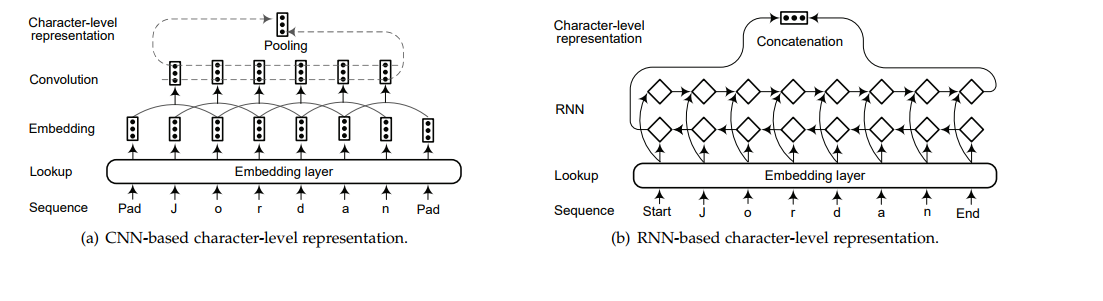
\includegraphics[width = 10cm]{Imagenes/charEmb.png}
	\caption{Modelos basados en CNN y RNN para la extracci\'on de la representaci\'on de la palabra a nivel de caracteres.}\label{fig:charLevel}
\end{figure}

Tambi\'en existen representacioes h\'ibridas donde adem\'as de representaciones a nivel de palabras y caracteres, incorporan informaci\'on adicional como los \emph{gazetters}~\cite{huang2015bidirectional} y similaridad l\'exica~\cite{ghaddar2018robust}. A\~nadir informaci\'on extra puede mejorar el desempe\~no de \textbf{NER} pero a su vez puede da\~nar la generalizaci\'on de estos sistemas. Un ejemplo de esto es el modelo \emph{BiLSTM-CRF} presentado en~\cite{huang2015bidirectional} donde 4 tipos de rasgos fueron utilizados: \emph{spelling features}, \emph{context features}, \emph{word embeddings} y \emph{gazetters}, los resultados muestran que el uso de rasgos extras como los \emph{gazetters} incrementan la precisi\'on del sistema. El art\'iculo~\cite{wei2016disease} presenta un sistema de redes neuronales basado en \emph{CRF} para el reconocimiento y normalizaci\'on de nombres de enfermedades; este sistema utiliza \emph{word embeddings} incluyendo, \emph{POS tags}, \emph{chunking} y rasgos correspondientes a la forma de las palabras (i.e, diccionarios y rasgos morfol\'ogicos). Otros trabajos con representaciones h\'ibridas son~\cite{lin2017multi},~\cite{aguilar2019multi},~\cite{jansson2017distributed},~\cite{moon2018multimodal}. Actualmente uno de los modelos de representaci\'on de lenguajes m\'as utilizados es \emph{Bidirectional Encoder Representations from Transformers}(\textbf{BERT})~\cite{devlin2018bert} que utiliza modelos de lenguaje enmascarados para permitir el pre-entrenamiento de representaciones bidireccionales. Para un \emph{token} determinado, su representaci\'on es compuesta por su posici\'on correspondiente, segmento y \emph{token embeddings}.


\subsection{Redes Neuronales Convolucionales}
Las CNN son un algoritmo de aprendizaje de m\'aquina, donde desde lo m\'as b\'asico pueden ser vistas como una especie de red neuronal que utiliza muchas copias del mismo neur\'on. Esto permite a la red tener muchos neurones y expresar computacionalmente enormes modelos mientras conserva el n\'umero actual de par\'ametros. Las CNN se utilizan fundamentalmente en el procesamiento de im\'agenes, pero forman parte tambi\'en del estado del arte del procesamiento de lenguaje natural actualmente.

Su funcionamiento se basa fundamentalmente en la operaci\'on de convoluci\'on. La misma utiliza una ventana denominada \emph{kernel}. Un \emph{kernel} es una matriz pequeña cuyos valores son los par\'ametros de las capas convolucionales. La misma se desliza por el vector de entrada (una oraci\'on por ejemplo), efectuando una operaci\'on de producto escalar para producir la salida. La distancia entre cada salto del kernel se denomina \emph{stride}.(PONER PAPER DE EXPLICACION DE UNA CNN) 

Un ejemplo de un acercamiento a partir de \textbf{CNN} al problema de \textbf{NER} es el presentado en~\cite{collobert2011natural} donde una palabra es etiquetada teniendo en consideraci\'on la oraci\'on completa. Cada palabra en la secuencia de entrada se representa a partir de un vector $N-dimensional$ despu\'es de la fase de representaci\'on de la entrada. Luego, una \textbf{CNN} es usada para producir rasgos locales alrededor de cada palabra y el tama\~no de la salida de las capas convolucionales depende en el n\'umero de palabras en la oraci\'on. El vector de rasgos global se construye combinando los vectores de rasgos locales extra\'idos por las capas convolucionales. La dimensi\'on del vector global de salida es fija en orden de aplicar subsequent affine layers. Dos acercamientos son los m\'as utilizados para extraer rasgos globales: el m\'aximo o el promedio sobre la posici\'on (i.e time step) en la oraci\'on. Finalmente, este vector de rasgos global de dimensi\'on fija es la entrada del decodificador de etiquetas para computar la distribuci\'on de las puntuaciones para cada una de la etiquetas. Siguiendo el trabajo~\cite{collobert2011natural} se encuentra el sistema \textbf{Bio-NER} para el reconocimiento de entidades en textos biom\'edicos~\cite{yao2015biomedical}. Otros art\'iculos utilizando \textbf{CNN} para el problema de \textbf{NER} son~\cite{strubell2017fast},~\cite{zhou2017joint}.

\subsection{Redes Neuronales Recurrentes}

Las redes neuronales recurrente son un algoritmo de aprendizaje de m\'aquinas, donde las conexiones entre los nodos forman un grafo dirigido dentro de una secuencia temporal. A diferencia de las \emph{Feedforward Neural Networks}, las \textbf{RNN} pueden utilizar su estado interno (memoria) para procesar secuencias de entrada. Lo cual hace que se utilice esencialmente en tareas como segmentaci\'on, reconocimiento de escritura a mano, reconocimiento del habla, extracci\'on y clasificaci\'on de palabras claves y extracci\'on de relaciones entre palabras claves en una oraci\'on. La red neuronal recurrente incluye conexiones que apuntan "hacia atr\'as", una especie de retroalimentaci\'on entre las neuronas dentro de las capas, a diferencia de otras redes cuya funci\'on de activaci\'on solo act\'ua en una direcci\'on.(PONER REFERENCIA DE DONDE SE EXPLIQUEN LAS RNN). En la figura~\ref{fig:RNN} se aprecia una arquitectura para \textbf{NER} basada en \textbf{RNN}.

\begin{figure}[h!]
	\centering
	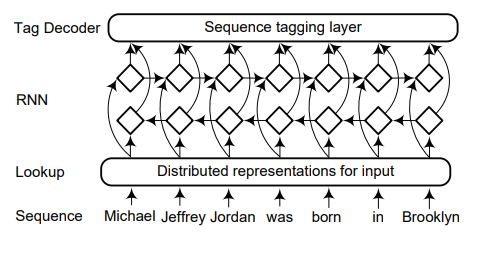
\includegraphics[width = 10cm]{Imagenes/RNN_Arquitecture.png}
	\caption{Modelo para \textbf{NER} basado en \textbf{RNN}.}\label{fig:RNN}
\end{figure}

Las \textbf{RNN} junto sus variantes tales como \emph{Gated Recurrent Unit} (\textbf{GRU}) y \emph{Long Short Term Memory} (\textbf{LSTM}), han demostrado notables logros en la modelaci\'on de datos secuenciales. En particular, las \textbf{RNN} bidireccionales hacen uso eficientemente de informaci\'on pasada (v\'ia \emph{forward states}) e informaci\'on futura (v\'ia \emph{backward states}) para un espec\'ifico time frame~\cite{huang2015bidirectional}. Por lo tanto, un \emph{token} codificado por una \textbf{RNN} bidireccional va a contener informaci\'on de toda la oraci\'on. El trabajo de \emph{Huang et al.}\cite{huang2015bidirectional} est\'a entre los primeros en utilizar una arquitectura de \textbf{BiLSTM-CRF} para el etiquetado de secuencias. Siguiendo este trabajo muchos trabajos como~\cite{lample2016neural},~\cite{chiu2016named},~\cite{nguyen2016toward},
\cite{zhai2017neural},~\cite{zhou2017joint},~\cite{ma2016end},~\cite{tran2017named},~\cite{rei2016attending},~\cite{wei2016disease},~\cite{lin2017multi} aplican \textbf{BiLSTM} como la arquitectura b\'asica para codificar la informaci\'on de contexto. \emph{Yang et al.}~\cite{yang2016multi} utiliz\'o profundas \textbf{GRU} tanto a nivel de caracteres como de palabras para codificar la morfolog\'ia y la informaci\'on contextual. Trabajos recientes como~\cite{katiyar2018nested},~\cite{ju2018neural} dise\~naron una red neuronal basada en \textbf{LSTM} para el reconocimiento de entidades nombradas que se encuentran solapadas. Particularmente el trabajo~\cite{ju2018neural} propuso un modelo de redes neuronales para identificar entidades solapadas apilando flat \textbf{NER} layers din\'amicamente hasta que ninguna entidad externa es extra\'ida. Cada flat \textbf{NER} layer emplea una \textbf{BiLSTM} para capturar contexto secuencial. El modelo mezcla las salidas de las capas de \textbf{BiLSTM} en el actual flat \textbf{NER} layer para construir nuevas representaciones para la detecci\'on de entidades para que sirvan de entrada a la siguiente flat \textbf{NER} layer.

\subsection{Redes Neuronales Recursivas}

Las redes neuronales recursivas son modelos adaptativos no lineales que son capaces de aprender informaci\'on estructurada profunda a partir de explorar una estructura dada en un orden topol\'ogico~\cite{li2018survey}. Las entidades nombradas est\'an altamente relacionadas a constituyentes lingu\'isticos como los sustantivos~\cite{li2017leveraging}. Sin embargo, un acercamiento t\'ipico para el etiquetado de secuencias toma en poca consideraci\'on la estructura de las frases de las oraciones. \emph{Li et al.}~\cite{li2017leveraging} propuso clasificar cada nodo en una estructura constituyente para \textbf{NER}. Este modelo calcula recursivamente los vectores ocultos de estado de cada nodo y los clasifica seg\'un los vectores ocultos.

\subsection{Neural Languaje Model}

Los modelos de lenguajes es una familia de modelos describiendo la generaci\'on de secuencias. Dada una secuencia de \emph{tokens} $(t_1, t_2, ..., t_N)$, un forward language model computa la probabilidad de la secuencia a partir de modelar la probabilidad del \emph{token} $t_k$ dado su historia $(t_1,...,t_{k-1})$~\cite{peters2017semi}.

\begin{equation}
	p(t_1, t_2, ..., t_N) = \prod_{k=1}^{N} p(t_k | t_1, t_2, ..., t_{k-1})
\end{equation}


A backward language model es similar a un forward language model, excepto que corre por la secuencia en orden reverso, prediciendo el \emph{token} dado el contexto futuro:

\begin{equation}
p(t_1, t_2, ..., t_N) = \prod_{k=1}^{N} p(t_k | t_{k + 1}, t_{k + 2}, ..., t_N)
\end{equation}

Para los modelos de lenguajes neuronales, la probabilidad del \emph{token} $t_k$ puede ser calculada a partir de la salida de una \textbf{RNN}. En cada posici\'on $k$, se puede obtener dos representaciones dependientes del contexto (forward and backward) y entonces combinarlas como el embedding de lenguaje del modelo final para el \emph{token} $t_k$. Este modelo de lenguaje aumentado ha sido emp\'iricamente verificado como \'util en numerosas tareas de etiquetado~\cite{peters2017semi},~\cite{peters2018deep},~\cite{rei2017semi},~\cite{liu2018efficient},~\cite{liu2018empower}. Particularmente en los trabajos~\cite{liu2018efficient},~\cite{liu2018empower} se utiliza una arquitectura conocida como \textbf{LM-BiLSTM-CRF} donde el modelo de lenguaje y el modelo de etiquetado de secuencia comparten la misma capa a nivel de caracteres en una forma \emph{multi-task}. Los vectores de los \emph{embeddings} a nivel de caracteres, los \emph{word embeddings} pre-entrenados y la representaci\'on del modelo de lenguaje son concatenados y sirven de entrada para las \textbf{LSTM} a nivel de palabra. \emph{Peter et al.}~\cite{peters2018deep} propone la representaci\'on \textbf{ELMo} que es computada encima de dos capas de modelos de lenguaje bidireccional con convoluciones de caracteres. Este nuevo tipo de representaci\'on contextualizada profunda de una palabra es capaz de modelar caracter\'isticas complejas del uso de la palabra (sem\'antica y sintaxis), as\'i como el uso de variaciones a trav\'es de distintos contextos lingu\'isticos (polysemy). La figura~\ref{fig:LM} muestra las diferencias entre las arquitecturas de los modelos pre-entrenados.

\subsection{Deep Transformer}

Modelos neuronales para el etiquetado de secuencias est\'an t\'ipicamente basados en complejas \textbf{CNN} o \textbf{RNN} que consisten de un \emph{encoder} y un \emph{decoder}. Los \emph{Transformers} propuestos por~\cite{vaswani2017attention} son una arquitectura \emph{sequence-to-sequence}(\textbf{Seq2Seq}) que hacen uso de los mecanismos de atenci\'on, los cuales deciden en cada paso, que partes de la secuencia son relevantes a partir de las capas de \textbf{self-attention} o \textbf{multi-headed-attention}. Experimentos en varios tasks~\cite{kitaev2018constituency},~\cite{liu2018generating} muestran que los \emph{Transformers} son superiores en calidad y adem\'as requieren de significativamente menos tiempo para entrenar. Basado en \emph{Transformers} est\'a~\cite{radford2018improving} que propone \emph{Generative Pretrained Transformer} (\textbf{GPT}) para la tarea del entendimiento de lenguaje. A diferencia de \textbf{GPT} que es una arquitectura de izquierda a derecha, se encuentra \textbf{BERT}~\cite{devlin2018bert}. La representaci\'on pre-entrenada de \textbf{BERT} puede ser fine-tune con una capa de salida adicional para un amplio rango de tareas, incluyendo \textbf{NER}. En la figura~\ref{fig:transformer} se aprecia la arquitectura base de los Transformers.

\begin{figure}[H]
	\centering
	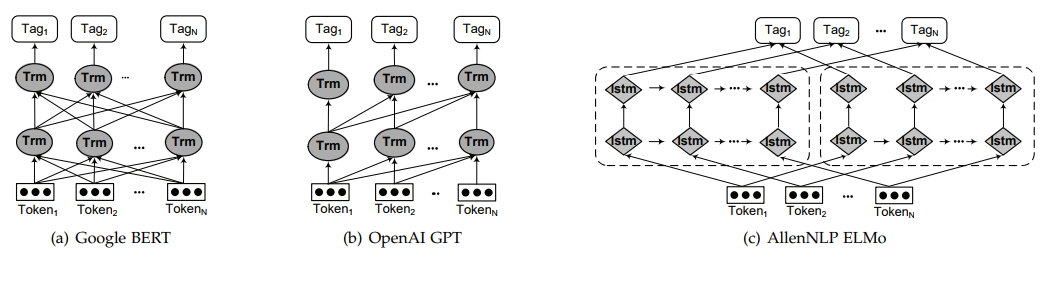
\includegraphics[width = 10cm]{Imagenes/LM.png}
	\caption{Diferencias entre las arquitecturas de los modelos pre-entrenados. \textbf{BERT} usa un Transformer bidireccional (abreviado como \textbf{Tmr}). \textbf{OpenAI GPT} usa un Transformer de izquierda a derecha. \textbf{ELMo} usa la concatenacion de dos LSTM entrenadas independientemente de izquierda a derecha y de derecha a izquierda respectivamente}\label{fig:LM}
\end{figure}

\begin{figure}[h!]
	\centering
	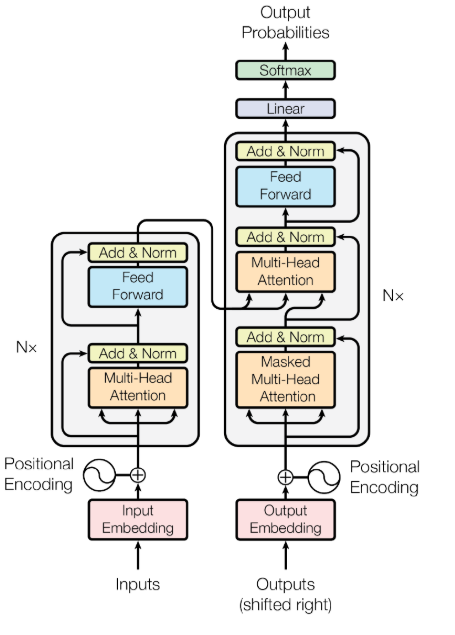
\includegraphics[width = 10cm]{Imagenes/Transformer.png}
	\caption{Arquitectura Transformer.}\label{fig:transformer}
\end{figure}


\subsection{Arquitecturas de Decodificaci\'on de Etiquetas}

La decodificaci\'on de etiquetas es la etapa final en un modelo de \textbf{NER}. Toma como entrada las representaciones dependientes del contexto y produce una secuencia de etiquetas correspondiente a la secuencia de entrada.

Una capa para la decodificaci\'on de etiquetas es la \emph{multi-layer Perceptron + Softmax} donde la tarea del etiquetado de secuencias es tratada como un problema de clasificaci\'on m\'ultiple. La etiqueta para cada palabra es independientemente predicha basado en las representaciones dependientes del contexto sin tener en cuenta sus vecinos. Ejemplos de modelos para \textbf{NER} que usan esta capa para la decodificaci\'on son~\cite{strubell2017fast},~\cite{li2017leveraging},\cite{xu2017local}.

Otra capa son los \emph{Conditional Random Fields} (\textbf{CRF}) que es un campo aleatorio globalmente condicionado en las observaciones de la secuencia~\cite{lafferty2001conditional}. Los \textbf{CRF} son un modelo discriminativo que modela los l\'imites de decisi\'on entre las diferentes clases en las que se puede clasificar un elemento de una secuencia.

Los \textbf{CRF} han sido usado ampliamente en aprendizaje supervisado basado en rasgos. Muchos modelos de \textbf{NER} utilizan \textbf{CRF} como su decodificador de etiquetas, como ejemplo de un \textbf{CRF} encima de una capa \emph{LSTM} es~\cite{huang2015bidirectional},~\cite{peters2018deep} y encima de una \textbf{CNN} es~\cite{collobert2011natural},~\cite{yao2015biomedical}. Sin embargo, \textbf{CRF} no puede hacer un uso completo de la informaci\'on a nivel de segmentos porque las propiedades internas de los segmentos no pueden ser completamente codificadas con representaciones a nivel de palabra~\cite{li2018survey}. \emph{Zhuo et al.}~\cite{zhuo2016segment} propuso el \emph{gated recursive semi-markov CRF}, el cual directamente modela los segmentos en vez de palabras y automaticamente extrae rasgos a nivel de segmentos a trav\'es de una \emph{gated recursive convolutional neural network}. Recientemente \emph{Ye and Ling}~\cite{ye2018hybrid} propusieron un h\'ibrido \emph{semi-Markov CRF} para el etiquetado de secuencias a partir de redes neuronales. Este acercamiento adopta segmentos en vez de palabras como su unidad b\'asica para la extracci\'on de rasgos y modelado de transiciones. Las etiquetas a nivel de palabras son utilizadas para derivar puntuaciones de segmentos. As\'i que este acercamiento es capaz de subir el nivel tanto de la informaci\'on a nivel de palabra como a nivel de segmento para cada c\'alculo de la puntuaci\'on de un segmento.

Algunos estudios como~\cite{shen2017deep},~\cite{nguyen2016toward},~\cite{zheng2017joint},~\cite{zhou2017joint},~\cite{vaswani2016supertagging} han explorado \textbf{RNN} para la decodificaci\'on de etiquetas. \emph{Shen et al.}~\cite{shen2017deep} report\'o que las \textbf{RNN} superan a los \textbf{CRF} y son m\'as r\'apidas de entrenar cuando el n\'umero de tipos de entidades es grande.

\emph{Pointer Networks} utilizan \textbf{RNNs} para aprender la probabilidad condicional de una secuencia de salida con elementos que son \emph{tokens} discretos correspondientes a las posiciones en la secuencia de entrada~\cite{vinyals2015pointer}. Representan diccionarios de tama\~nos variables usando la distribuci\'on de probabilidad \emph{softmax} como un puntero. \emph{Zhai et al.}~\cite{zhai2017neural} aplic\'o por primera vez \emph{Pointer Networks} para producir secuencia de etiquetas.

En la figura~\ref{fig:tagDec} se aprecia las diferencias entre algunos de los decodificadores de etiquetas antes presentados.

\begin{figure}[h!]
	\centering
	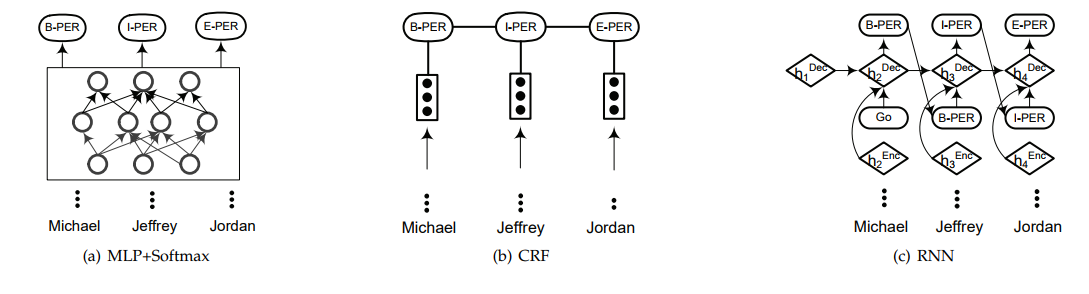
\includegraphics[width = 10cm]{Imagenes/TagDecoders.png}
	\caption{Diferencias entre 3 decodificadores de etiquetas: \textbf{MLP + Softmax}, \textbf{CRF}, \textbf{RNN}.}\label{fig:tagDec}
\end{figure}


\subsection{T\'ecnicas de Deep Learning para NER}
En las \'ultimas secciones se ha hecho un resumen de las t\'ipicas arquitecturas para enfrentar el problema de \textbf{NER}. En esta secci\'on presentamos t\'ecnicas de \textbf{Deep Learning} recientemente aplicadas a \textbf{NER}. Entre estas se incluyen \emph{deep multi-task learning}, \emph{deep transfer learning}, \emph{deep active learning}, \emph{deep reinforcement learning}, \emph{deep adversarial learning}, y \emph{neural attention}.

\subsubsection{Deep Multi-Task Learning}

\emph{Multi-task learning} es un acercamiento que aprende un conjunto de tareas juntas~\cite{caruana1997multitask}. Si se consideran las relaciones entre las diferentes tareas, se espera que los algoritmos de \emph{multi-task learning} consigan mejores resultados que aquellos que aprenden una tarea individualmente~\cite{li2018survey}.

Trabajos como~\cite{collobert2011natural} han entrenado modelos para conjuntamente enfrentar las tareas de \textbf{POS}, \textbf{Chunk}, \textbf{NER} y \textbf{SRL}. El trabajo de \emph{Yang et al.}~\cite{yang2016multi} propuso un modelo conjunto \emph{multi-task}, para aprender regularidades espec\'ificas del lenguaje, entrenando conjuntamente en las tareas de \textbf{POS}, \textbf{NER}, \textbf{Chunk}. La idea del \emph{multi-task learning} ha sido aplicada adem\'as para entrenar modelos conjuntos para \textbf{NER} y a su vez la extracci\'on y clasificaci\'on de relaciones~\cite{zheng2017joint},~\cite{zhou2017joint} o adem\'as modelar \textbf{NER} como dos subtareas relacionadas, la segmentaci\'on de entidades y la predicci\'on de las categor\'ias  de las entidades~\cite{aguilar2019multi},~\cite{peng2016multi}. En el dominio biom\'edico, debido a las diferencias en los distintos conjuntos de datos, la tarea de \textbf{NER} en cada conjunto de datos es considerada una tarea en una configuraci\'on \emph{multi-task}~\cite{crichton2017neural},~\cite{wang2019cross}. La principal suposici\'on es que los diferentes conjuntos de datos comparten la misma informaci\'on a nivel de caracteres y de palabras, entonces \emph{multi-taks learning} es aplicado para hacer un uso m\'as eficiente de los datos y alentar al modelo a aprender representaciones m\'as generalizadas.


\subsubsection{Deep Transfer Learning}

\emph{Transfer Learning} apunta a lograr un mejor desempe\~no de una tarea de aprendizaje de m\'aquina en un dominio espec\'ifico tomando ventaja del conocimiento aprendido del dominio fuente~\cite{pan2009survey}. En \textbf{NLP}, \emph{trasnfer learning} es tambi\'en conocido como adaptaci\'on de dominio. En las tareas de \textbf{NER} el acercamiento tradicional es a trav\'es de los algoritmos de \emph{bootstrapping}~\cite{jiang2007instance}, \cite{wu2009domain}. Recientemente, nuevos acercamientos como~\cite{pan2013transfer},~\cite{lee2017transfer} han propuesto usar redes neuronales profundas for accross-domain \textbf{NER}.

En las configuraciones de \emph{transfer learning} diferentres modelos neuronales comunmente comparten diferentes partes de los par\'ametros del modelo entre la tarea fuente y la tarea objetivo. \emph{Yang et al.}~\cite{yang2017transfer} fue el primero en investigar la transferibilidad de las diferentes capas de representaci\'on, entonces presentaron 3 diferentes arquitecturas para compartir par\'ametros entre escenarios de \emph{cross-domain}, \emph{cross-lingual} y  \emph{cross-application}. En particular si dos tareas tienen conjuntos de etiquetas mapeables, entonces hay una capa de \textbf{CRF} compartida, en otro caso cada tarea tiene su propia capa de \textbf{CRF}. Otros trabajos de \emph{trasnfer learning} en \textbf{NER} son~\cite{von2017transfer},~\cite{zhao2018improve},~\cite{lin2018neural},~\cite{giorgi2018transfer}.

\subsubsection{Deep Active Learning}

La idea esencia detr\'as de \emph{deep active learning} es que un algoritmo de aprendizaje de m\'aquina pueda desempe\~narse mejor con una cantidad substancial menor de datos de entrenamiento, si se permite elegir los datos con los que entrenar\'a~\cite{settles2012active}. Aprendizaje profundo requiere una gran cantidad de datos de entrenamiento que es costoso de obtener. Por lo tanto, combinando aprendizaje profundo con \emph{active learning} se espera que se reduzca el esfuerzo de anotaci\'on de los datos.

Entrenamiento con \emph{active learning} procede en m\'ultiples rondas. Sin embargo, los esquemas tradicionales de \emph{active learning} son costosos para aprendizaje profundo, porque despu\'es de cada ronda requiere un reentrenamiento completo del clasificador con nuevos datos anotados. Precisamente porque el reentrenamiento desde el inicio no es pr\'actico para aprendizaje profundo \emph{Shen et al.}~\cite{shen2017deep} propuso un entrenamiento incremental para \textbf{NER} con cada \emph{batch} de nuevas etiquetas. La idea, es mezclar nuevos ejemplos anotados con algunos ya existentes, y actualizar los pesos de la red neuronal para un n\'umero peque\~no de \emph{epochs}, antes de consultar por etiquetas en una nueva ronda. Espec\'ificamente, al inicio de cada ronda, el algoritmo de \emph{active learning} elige oraciones para ser anotadas, que pertenecen a un grupo de oraciones predefinido. Los par\'ametros del modelo son actualizados por el entrenamiento en el conjunto de datos aumentado, despu\'es de recibir las anotaciones seleccionadas.

\subsubsection{Deep Reinforcement Leaarning}

\emph{Reinforcement Learning} es una rama del aprendizaje de m\'aquinas inspirada por la psicolog\'ia del comportamiento, que tiene que ver con c\'omo agentes de software toman acci\'on en el ambiente con el objetivo de maximizar alguna recompensa acumulativa~\cite{kaelbling1996reinforcement},~\cite{sutton1998introduction}. La idea es que el agente aprender\'a a partir de la interacci\'on con el ambiente y recibiendo recompensas por realizar acciones. Especifiamente el problema del \emph{reinforcement learning} puede ser formulado de la siguiente forma~\cite{hoi2018online}: el ambiente es modelado como una m\'aquina de estado estoc\'astica finita con entradas (acciones del agente) y salidas (observaciones y recompensa del agente). Esto consiste en 3 componentes claves:
 
 \begin{enumerate}
 	\item La funci\'on de transici\'on de estados.
 	\item La funci\'on de observaciones (o sea, salida).
 	\item La funci\'on de recompensa.
 \end{enumerate}
 
El agente es tambi\'en modelado como una m\'aquina de estado estoc\'astica finita con entradas (observaciones y recompensas del ambiente) y salidas (acciones en el ambiente). Esto consiste en dos componentes: (i) una funci\'on de transici\'on de estado, y (ii) una funci\'on de salida. La meta final del agente es aprender una buena funci\'on de actualizaci\'on de estado intentando maximixar las recompensas acumuladas.

\emph{Narasimhan et al.}~\cite{narasimhan2016improving} model\'o la tarea de extracci\'on de informaci\'on como un proceso de decisi\'on de \emph{Markov} \textbf{MDP}, el cual din\'amicamente incorpora predicci\'on de entidades y provee de flexibilidad para elegir las siguiente consulta de b\'usqueda de un conjunto de alternativas autom\'aticamente generado.

\subsection{Deep Adversarial Learning}

\emph{Adversarial Learning} es el proceso de explic\'itamente entrenar un modelo en ejemplos adversariales. El prop\'osito es hacer el modelo m\'as robusto contra ataques o reducir sus test error on clean inputs. \emph{Adversarial networks} aprenden a generar a partir de una distribuci\'on de entrenamiento a trav\'es de un juego de dos jugadores: una red genera candidatos (\emph{generative network}) y la otra los eval\'ua (\emph{discriminative network}). T\'ipicamente, la red generativa aprende a mapear de un espacio latente a una distribuci\'on particular de los datos de inter\'es, mientras que la red discriminativa discrimina entre los candidatos generados por el generador e instancias de la distribuci\'on de datos del mundo real~\cite{goodfellow2014generative}.

\emph{Dual adversarial transfer network} (\textbf{DATNet}), propuesto en~\cite{zhou2018datnet} apunta a lidiar con el problema de los bajos recursos en \textbf{NER}. Los autores preparan una muestra adversarial a\~nadiendole a la muestra original una perturbaci\'on acotada por una peque\~na norma $\epsilon$ para maximizar la funci\'on de p\'erdida como sigue:

\begin{equation}
	\eta_x = arg \ max_{\eta:\lVert \eta \rVert_2 \ \leq \ 2 } \ l(\theta; x + \eta)
\end{equation}

donde $\theta$ es el conjunto actual de par\'ametros del modelo, $\epsilon$ puede ser determinado en el conjunto de validaci\'on. Un ejemplo adversarial es construido por $x_{adv} = x + \eta_x$. El clasificador es entrenado en la mezcla de los ejemplos originales y los adversariales para mejorar la generalizaci\'on.


\subsection{Neural Attention}

El mecanismo de \emph{attention} en una red neuronal es basado en el mecanismo de atenci\'on virtual del humano~\cite{britz2016attention}. El mecanismo de \emph{neural attention} permite a las redes neuronales la habilidad de enfocarse en un subconjunto de sus entradas. Aplicando mecanismos de atenci\'on, un modelo de \textbf{NER} puede capturar los elementos m\'as informativos de las entradas. 

Existen muchas formas de aplicar el mec\'anismo de atenci\'on en las tareas de \textbf{NER}. \emph{Rei et al.}~\cite{rei2016attending}, aplic\'o el mecanismo de atenci\'on para din\'amicamente decidir cu\'anta informaci\'on utilizar de una componente a nivel de caracteres o palabras en un modelo de \textbf{NER} \emph{end-to-end}. \emph{Zukov-Gregoric et al.}~\cite{zukov2017neural} explor\'o el mecanismo de \emph{self-attention} en \textbf{NER}, donde los pesos son dependientes de una sola secuencia.

\section{Extracción de Relaciones}

Dada una oración $S$ con dos entidades señaldas $\langle e_1,e_2 \rangle$, la tarea de la extracción de relaciones consiste en identificar la relación semántica que se establece entre $e1$ y $e2$ en el contexto de $S$, seleccionada de un conjunto predefinido de relaciones candidatas~\cite{hendrickx2009semeval}.
Esta tarea se puede estructurar como un problema de clasificación multiclase en el que la salida esperada es una de múltiples clases predefinidas, incluyendo una clase ficticia para cuando la supuesta relación no aparece entre dichas clases~\footnote{Esta clase ficticia es referida como \textit{other} o \textit{none}.}.

En años pasados, la literatura registra dos enfoques fundamentales para resolver este problema: los métodos basados en rasgos~\cite{kambhatla2004combining, boschee2005automatic, guodong2005exploring, grishman2005nyu, jiang2007systematic, chan2010exploiting, rink2010utd, sun2011semi, rink2010utd, nguyen2014employing} y los métodos basados en \textit{kernels}~\cite{zelenko2003kernel, culotta2004dependency, bunescu2005shortest, qian2008exploiting, nguyen2009convolution, sun2014feature}, los cuales se diferencian en la forma en que representan las relaciones entre las entidades en el contexto de una oración.

\subsection{Enfoques basados en rasgos}

Los métodos basados en rasgos convierten la entrada del problema en una representación vectorial $(f_1,f_2,\dots,f_N)$.
Cada una estas componentes constituye una característica que hipotéticamente es efectiva para discriminar la existencia de relaciones entre las entidades.
Con esta representación, son entrenados algoritmos de aprendizaje de máquina estadístico como SVM y Clasificador de Máxima Entropía~(MEC)~\cite{maxentropy}.
Las características seleccionadas pueden tener naturaleza léxica, sintáctica o semántica.

De alguna forma u otra, todos los modelos incluyen información referente a las palabras de la oración.
La forma más simple de obtener esta representación es un índice que identifique la palabra dentro un vocabulario predeterminado.
No obstante, en trabajos más recientes se ha explorado el uso de representaciones vectoriales de las palabras, inducidas por modelos del lenguaje previamente entrenados en otras tareas~\cite{nguyen2014employing}.
Una de estas representaciones son los \textit{embeddings} de palabras.

En una metodología general, enfrentar la tarea de extracción de relaciones usualmente implica que anteriormente se hizo un análisis, manual o automático, de las entidades presentes en el texto y el tipo de las mismas. 
Existe una variedad de trabajos que validan la utilidad de esta información, ya que permite por ejemplo, restringir el dominio de algunas relaciones a ciertos tipos de entidades~\cite{kambhatla2004combining, boschee2005automatic, guodong2005exploring, jiang2007systematic, chan2010exploiting}.

Como complemento de la información que aportan las entidades señaladas, también se ha evaluado el uso de sus contextos.
Dígase las palabras que son adyacentes, palabras entre las menciones o palabras antes y depués de las menciones~\cite{guodong2005exploring, chan2010exploiting, sun2011semi, nguyen2014employing}.

Han probado ser efectivos rasgos extraídos de las estructuras que resultan del análisis sintáctico~(parsing) de la oración.
Entre estas estructuras se encuentran los árboles de constituyentes~(o sintácticos) y los de dependencias.
Los árboles de constituyentes capturan la estructura sintáctica de la oración de acuerdo a una gramática estructurada por frases~(o gramáticas de constituyentes)~\cite{chomsky2002syntactic}.
Entre tanto, los árboles de dependencias describen la estructura sintáctica de la oración solamente en términos de las palabras de la misma y un conjunto asociado de relaciones gramaticales binarias que se establecen entre las ellas~\cite{tesniere2015elements}.

Otro recurso sintáctico empleado son las etiquetas de parte de la oración~(referidas como \textit{POS-tag} por sus siglas en inglés), que describen la función gramatical que tiene cada palabra dentro de la oración.
En el año 2004, \textit{Kambhatla}~\cite{kambhatla2004combining} propuso utilizar el camino en el árbol de parsing sintáctico, así como la palabra en la que cada entidad era dependiente, la función gramatical de la frase que las une y su \textit{POS-tag}.
Otras combinaciones de las cabeceras y dependientes de las entidades, sus funciones gramaticales y \textit{POS-tag} fueron analizadas por \textit{GuoDong} en 2005~\cite{guodong2005exploring}~\footnote{Varios de los trabajos citados en este estudio tomaron este conjunto de características como base de sus modelos}.

Debido a la naturaleza semántica que pueden tener las relaciones a extraer, las fuentes externas de información semántica constituyen otro amplio espacio de características relevantes.
Una de la fuentes más utilizadas es el diccionario el hiperórimos de \textit{WordNet}~\footnote{http://wordnet.princeton.edu/}~\cite{guodong2005exploring, rink2010utd}.
El trabajo realizado por \textit{Rink y Harabagiu} en 2010~\cite{rink2010utd} investiga la influencia de otra variedad de fuentes externas de información semántica como: NomLex-Plus~\footnote{http://nlp.cs.nyu.edu/meyers/NomBank.html}, VerbNet~\footnote{http://verbs.colorado.edu/ mpalmer/projects/verbnet.html}, N-gramas de Google~\footnote{Disponible desde LDC como LDC2006T13} y TextRunner~\cite{yates2007textrunner}.
En 2010, \textit{Chan y Roth}~\cite{chan2010exploiting} propusieron utilizar información extraída de \textit{Wikipedia}.

\subsection{Enfoques basados en kernels}

Los métodos basados en \textit{kernels}, por su parte, pueden prescindir de representaciones complejas de las estructuras de una oración. 
Se apoyan en funciones con características especiales denominadas \textit{kernels}.
Un \textit{kernel} $K$ sobre un espacio vectorial $E$ es una función binaria $K:E\times E\rightarrow [0,\infty)$ simétrica y semidefinida positiva.
Se puede demostrar que una función de \textit{kernel} calcula implícitamente el producto escalar de vectores que representan a los objetos en espacios de grandes~(y potencialmente infinitas) dimensiones.
Esto es, para todo \textit{kernel} $K$, $\exists f:E\rightarrow T$, tal que $K(x,y)=g(f(x),f(y))$, con $g:T\times T \rightarrow R$ un producto escalar definido sobre $T$ y $x,y\in E$. También se cumple el recíproco de este teorema.
Esta propiedad de los \textit{kernels} le permite a los algoritmos de aprendizaje representar, aunque implícitamente, los objetos en espacios de grandes dimensiones y computar su producto escalar eficientemente como medida de similaridad.

Cuando un algoritmo de aprendizaje puede ser reescrito en términos de una función de \textit{kernel} sustituyendo al producto escalar, se le denomina algoritmo dual.
Existen diversos algoritmos que hacen uso de las facilidades que presentan los \textit{kernel}.
Entre ellos se encuentran SVM y Perceptrón de Kernel~\cite{aizerman1964theoretical}.

Desde el punto de vista del diseño de algoritmos de aprendizaje de máquinas, este enfoque centra su atención en la definición de \textit{kernels} que midan correctamente la similaridad entre los objetos, delegando el trabajo de obtener una representación adecuada para ello a la función escogida.
Estos estudios proponen deficiones de \textit{kernels} sobre estructuras como: árboles de \textit{parsing} sintáctico~\cite{zelenko2003kernel, zhao2005extracting, zhang2006composite, zhou2007tree}, árboles de dependencias~\cite{culotta2004dependency, bunescu2005shortest, zhao2005extracting} y subsecuencias del texto~\cite{zhao2005extracting, mooney2006subsequence}, por citar algunos ejemplos.

Rara vez estas propuestas son puramente basadas en \textit{kernels}.
Se ha explorado la posibilidad de enriquecer las representaciones con propiedades típicas de enfoques basados en características~\cite{culotta2004dependency, bunescu2005shortest, zhang2006composite, zhao2005extracting}.

\subsection{Enfoques basados en aprendizaje profundo}

Con el desarrollo de las técnicas de aprendizaje profundo, los investigadores han explotado este nuevo enfoque para enfrentar el problema de la extracción de relaciones.
Hasta este punto, los métodos para ello se concentraron en aprendizaje de máquinas estadístico y su desempeño dependía de la calidad de los rasgos extraídos, o de los \textit{kernels} definidos.
La mayoría de las propuestas se apoyaban de manera determinante, en técnicas de NLP que constituyen problemas parcialmente resueltos con cierto grado de error, como \textit{parsing} de dependencias, \textit{parsing} sintáctico, extracción de entidades y etiquetado en partes de la oración; lo cual conducía a una propagación del error.
Las capacidades de las técnicas de aprendizaje profundo para obtener representaciones complejas a partir de estructuras más simples, es la suposición esencial a la que responden los enfoques más modernos.

De manera general, estas técnicas se centran en obtener una representación vectorial de la oración teniendo en cuenta las entidades señaladas, la cual sirve de entrada a un clasificador multiclase que determina a cuál de las relaciones responde el par ordenado $\langle e_1,e_2\rangle$.
Usualmente este clasificador está constituído por un Perceptrón Multicapa~(MLP) con función de activación \textit{softmax}, que genera una distribución de probabilidades sobre las posibles relaciones.

En la literatura aparecen dos técnicas fundamentales empleadas con el fin de codificar la oración y el par de entidades en cuestión: Redes Neuronales Convolucionales~(CNN) y Redes Neuronales Recurrentes/Recursivas (RNN).

Los modelos que se apoyan en CNN~\cite{zeng2014relation, santos2015classifying, nguyen2015relation, xu2015semantic, huang2016attention, wang2016relation}, explotan la capacidad de las mismas para obtener representaciones de los elementos de una secuencia, contextualizados en una ventana centrada en cada elemento. En lo referente a las palabras de una oración, a estas ventanas se les denomina \textit{n-gramas}.
En su trabajo, \textit{Zeng et al}~\cite{zeng2014relation} proponen una CNN para capturar los rasgos de la oración y las entidades en cuestión.
Incluyen de manera adicional información de los \textit{tokens} adyacentes de cada palabra.
La representación final la obtienen mediante una operación de \textit{max-pooling} sobre el conjunto de vectores resultante de cada una de las ventanas de convolución.
La clasificación se obtiene mediante un MLP con activación \textit{softmax}, sobre el conjunto de relaciones más la clase ficticia \textit{none}.
Mientras este trabajo utiliza una convolución con ventanas fijas, \textit{Nguyen y Grishman}~\cite{nguyen2015relation} exploran el uso de varias convoluciones con distintos tamaños de ventana.
Por su parte, \textit{Santos et al}~\cite{santos2015classifying} proponen una alternativa para deshacerse de la clase ficticia.
Para ello entrenan el modelo minimizando una función de pérdida de \textit{ranking} definida por pares.
Esto trae como consecuencia una mejora notable de los resultados de su arquitectura tanto en precisión como en recobrado.

Los modelos basados en RNN~\cite{socher2012semantic, xu2015classifying, zhang2015bidirectional, ebrahimi2015chain, xiao2016semantic, lee2019semantic}, se apoyan en la posibilidades de las mismas para obtener representaciones vectoriales de estructuras secuenciales, así como de estructuras más complejas~(estructuras arbóreas por ejemplo), codificando de esta forma patrones globales y no necesariamente consecutivos dentro de la oración.
En 2015, \textit{Zhang et al}~\cite{zhang2015bidirectional} propusieron el uso de una red BiLSTM sobre la secuencia de \textit{tokens} para codificar cada palabra de la oración.
Obtienen una representación de las entidades señaladas mediante la concatenación de distintos rasgos léxicos y la salida correspondiente de la red BiLSTM.
Finalmente, combinan los rasgos obtenidos de la oración y las entidades mediante un MLP, cuya salida pasa por un clasificador \textit{softmax} para predecir la relación resultante.

Existen trabajos con propuestas que combinan el uso de CNN y RNN para distintas funciones~\cite{liu2015dependency, nguyen2015combining, cai2016bidirectional}.
En 2015, \textit{Nguyen y Grishman}~\cite{nguyen2015combining} exploraron el uso de aquitecturas que utilizan CNN y RNN, y experimentaron con distintos métodos de ensamblar los resultados de las mismas.
Por otro lado, \textit{Cai y Wang}~\cite{cai2016bidirectional} proponen una arquitectura convolucional/recurrente bidireccional~(BRCNN de acuerdo a sus siglas en inglés) que utiliza una capa CNN apilada sobre una capa LSTM.
Aplican esta arquitectura sobre la secuencia de entrada escogida~(construida a partir del camino en el árbol de dependencias) y sobre su reverso, para capturar la direccionalidad de las relaciones.

Como entrada para estos modelos puede ser utilizada la secuencia de palabras de la oración, sin ningún preprocesamiento~\cite{zeng2014relation, santos2015classifying, nguyen2015relation, huang2016attention, wang2016relation, xiao2016semantic}.
Lo anterior responde al supuesto de que la información más completa para resolver este problema se encuentra en la oración íntegra.
Estos son conocidos como modelos \textit{end-to-end}.
Para que el modelo no sea agnóstico de la posición de las entidades en la oración, se añade lo que se denomina características de posición, que codifican la posición relativa de cada \textit{token} de la oración con respecto a las entidades en cuestión~\cite{zeng2014relation, santos2015classifying, nguyen2015relation, zhang2015bidirectional,nguyen2015combining,huang2016attention, wang2016relation, xiao2016semantic, lee2019semantic}.

Otras variantes se apoyan en la suposición de que el árbol de dependencias de la oración de entrada condensa la información vital para resolver el problema, a la vez que desecha otras fuentes de desinformación.
En algunos casos se toma como representación de la entrada el camino en dicho árbol entre las entidades marcadas~\cite{socher2012semantic, xu2015classifying, hashimoto2015task, xu2015semantic, liu2015dependency, ebrahimi2015chain}.
En otros casos solo se añade información relevante extraída de esta estructura~\cite{zhang2015bidirectional}.
Resulta interesante el trabajo de \textit{Liu et al}, que definen una estructura que denominan Camino de Dependencias Aumentado~(ADP por sus siglas en inglés).
Esta estructura enriquece la representación del camino de dependencias incluyendo información de todo el subárbol del cual cada \textit{token} es raíz. 
Para extraer los rasgos de cada palabra en función de su correspondiente subárbol utilizan una RNN.
La información para resolver el problema de clasificación se obtiene luego a partir de una CNN sobre el ADP.

Para la representación de las palabras en una oración, ha demostrado ser efectivo el uso de \textit{embeddings} de palabras preentrenados en modelos generales del lenguaje.
Además, ha sido comprobado por la mayoría de los trabajos antes mencionados, que estos modelos ganan en efectividad cuando se enriquecen con características como: \textit{POS-tags}, información del tipo de las entidades señaladas, hiperónimos de \textit{WordNet} e información de las palabras adyacentes a las entidades señaladas.

Otro recurso que ha probado ser útil, no solo en esta sino en otras múltiples tareas de NLP, es la atención. 
En la tarea de extracción de relaciones se ha verificado que incluir niveles de atención sobre las palabras de la oración en función de las entidades señaladas, mejora la efectividad de los modelos, ya que ayuda a descartar información no relevante en la representación escogida~\cite{huang2016attention, wang2016relation, xiao2016semantic, lee2019semantic}.
La propuesta de \textit{Huang y Shen}~\cite{huang2016attention}, utiliza un mecanismo de atención sobre objetos heterogéneos, dígase la oración y las dos entidades en cuestión.
Con esto persiguen el objetivo de brindarle al modelo la capacidad de determinar qué partes de la oración son más influyentes con respecto a las dos entidades de interés.
\textit{Wang et al}~\cite{wang2016relation} consideran el uso de distintos niveles de atención.
Un nivel primario sobre la oración con respecto a las dos entidades en cuestión.
Sobre la secuencia se resultante aplican una operación de convolución para capturar información contextual, seguida por una operación de \textit{max-pooling}.
Utilizan luego un nivel secundario de atención para determinar la características resultantes de la convolución más relevantes para la clasificación de la relación .
\textit{Xiao y Liu}~\cite{xiao2016semantic} proponen el uso de dos BiLSTM apiladas con capas de atención intercaladas para descartar información irrelevante que aparece cuando se utiliza como entrada la oración completa.
Para capturar información referente a la relación mencionada, dividen la codificación obtenida por las BiLSTM en tres contextos, resultantes de dividir la oración en los lugares donde aparecen ubicadas las entidades en cuestión.

Recientemente, el modelo preentrenado BERT ha tenido resultados satisfactorios en muchas tareas de NLP y la extracción de relaciones no está exenta de esto.
En 2019, \textit{Soares et al}~\cite{soares2019matching} investigaron distintas arquitecturas para codificar una mención de una relación, todas construidas a partir de reoptimizar los parámetros del modelo BERT con objetivos de entrenamiento enfocados en la extracción de relaciones. 
Entre tanto \textit{Wu y He}~\cite{wu2019enriching} proponen un modelo para atacar el problema de la extracción de relaciones que combina información obtenida a partir de BERT con información extraída de las entidades señaladas.

\section{Enfoque Conjunto}

Comúnmente, las tareas de NER y ER son abordadas secuencialmente, con sistemas que extraen entidades y luego determinan qué relaciones existen entre las mismas.
Sin embargo, sistemas secuenciales de este tipo son propensos a propagar el error de una tarea hacia la siguiente.
Y, en dependencia de cómo estén implementados, puede que no exploten información relevante el uno del otro.
Es por ello que existe toda una línea de desarrollo orientada a explorar soluciones que resuelvan simultáneamente estas dos tareas~\cite{miwa2016end, li2017neural, bekoulis2018adversarial, bekoulis2018joint, li2019entity, nguyen2019end, giorgi2019end}.

La propuesta general se basa en definir una arquitectura que tenga salidas que le permitan resolver los dos problemas, similares a las descritas en secciones anteriores.
Con la particularidad de que se define una función de pérdida que considere ambas tareas, permitiendo así optimizar el modelo en función de resolver ambos problemas.
Además, algunas de las capas que codifican la información de entrada de estos modelos son compartidas en el cómputo de cada salida, permitiendo así el uso de información de una tarea en la resolución de la otra.

Algunas de estas propuestas, al igual que otras ya descritas, se apoyan en recursos externos de NLP, como son los \textit{parsers} de dependencias~\cite{miwa2016end, li2017neural}.
Esto, como se ha explicado, limita la efectividad de estos modelos en dominios donde dichas herramientas no funcionan como se esperaría~(e.g en dominios en los que no fueron entrenadas).

En respuesta a esto, se han desarrollado propuestas puramente \textit{end-to-end}, que no se apoyan en estos recursos~\cite{bekoulis2018joint}.
Este trabajo fue extendido con entrenamiento adversarial~\cite{bekoulis2018adversarial}.
En 2019, \textit{Nguyen y Verspoor}~\cite{nguyen2019end} propusieron un modelo similar, que usa adicionalmente un mecanismo de \textit{biaffine attention}~\cite{biaffineattention}.
\textit{Giorgi et al, 2019}~\cite{giorgi2019end} propusieron un modelo similar que incluye el uso del modelo preentrenado del lenguaje BERT, aliviando el costo de entrenamiento.
Por su parte, \textit{Li et al, 2019}~\cite{li2019entity}, enfocaron el problema con \textit{multi-turn} question answering, mediante un modelo de QA basado en BERT que respondía preguntas cuyas respuestas eran las las entidades y relaciones entre las mismas.
%===================================================================================

